\section{Dataset}

Our analysis is based on \TODO aliases from \TODO files on GitHub, collected in the period from \TODO to \TODO.

% TODO: graphic with collection pipeline, short description of process detailed below?
%We first collected \TODO files containing the word ``alias'' from GitHub, then we parsed these files, resulting in TODO alias definitions.
%The details of this process are described below.

\subsection{Data Collection}

Alias definitions can appear in any Shell script, but we anticipated that they would predominantly be found in personal configuration files (like \verb|.bashrc| or \verb|.bash_profile|).
While we did not want to focus exclusively on these personal configuration scripts, as we want to study the wide range of different alias uses, it is important that they are appropiately accounted for in order for our data to be representative.
Unfortunately, this rules out using some prominent existing datasets for our study:
The public GitHub archive on BigQuery\footnote{\url{https://bigquery.cloud.google.com/table/bigquery-public-data:github_repos.files}}, while containing over 1.5 TB of source code, only includes ``notable projects'' (presumably those with a certain number of stars on GitHub) that additionally have an explicit open source license. 
This leaves out many of the repositories we are interested in, as users sharing configuration scripts for personal use do not usually add a license file and their repositories are generally not ``notable''.\footnote{The data we have collected corroborates this: \TODO}
GHTorrent\footnote{\url{http://ghtorrent.org}}, another popular archive of GitHub data, only contains metadata but not file contents.

Therefore, we found it necessary to write our own tooling to directly collect the data from GitHub ourselves.
We used the GitHub Code Search API to find files written in Shell language\footnote{GitHub uses the Linguist library to classify source code: \url{https://github.com/github/linguist}} that contain the string \verb|alias|.

Alas, the GitHub Code Search API comes with its own set of limitations:
\begin{enumerate}
    \item only files smaller than 384 KB are searchable
    \item forks are not included
    \item requests are rate limited at 30 per minute and there are additional opaque abuse detection mechanisms that impose further restrictions in an unforseeable manner
    \item the number of results is limited to 1000 per search request
\end{enumerate}
The first two limitations do not really affect us, as we are mostly interested in smaller files and do not have to consider forks.
The rate limiting, while significantly slowing down the retrieval process, is also not a fatal obstacle.
The maximum number of returned search results, however, is a critical limitation.
To get around it, we wrote a Python tool called \verb|github-searcher|\footnote{\TODO: url/paper} that uses a stratified sampling technique to vastly increase the number of results we are able to retrieve.

The technique takes advantage of GitHub allowing code search queries to be conditioned on file sizes. 
For example, the query 
\begin{verbatim}
alias language:Shell size:101..200
\end{verbatim}
returns up to 1000 Shell language files containing the string ``alias'' that have a file size between 101 and 200 bytes (inclusive).
Repeating the search with 
\begin{verbatim}
alias language:Shell size:201..300
\end{verbatim}
returns up to 1000 files of a size between 201 and 300 bytes.
And so on.
Repeatedly searching with the same search term but different non-overlapping file size ranges allows us to significantly increase our sample of the overall population.
Another trick further improves on this: 
the API gives us an option to sort the results by most or least recently indexed;
if we run a search using a specific sort order, then we can effectively double the sample size by repeating the same search with the opposite sort order.
Thus we can get up to 2000 results per search per file size range.

Additionally, while GitHub doesn't allow us to retrieve more than a limited number of files per query, it does return the total count of files matching the query.
While this count is usually very erratic on broad searches, fluctuating wildly between repeated requests, it turns out to be fairly accurate for searches with a small number of results, such as those conditioned on a narrow range of file sizes.
This allows us to get a good estimate of the population, and how accurately our sample approximates it.

For this study, using the search term
\begin{verbatim}
alias language:Shell
\end{verbatim}
and the stratified sampling technique described above, we started by sampling in increments of 100 bytes, then re-sampled high-population areas with smaller size increments, down to a byte-by-byte sampling in certain cases.
In total, we collected \TODO files under \TODO KB from an estimated population of \TODO, achieving a sampling rate of \TODO\% (see \cref{fig:sampling}).
The file contents, together with repository metadata, were stored in an SQLite database (see \cref{fig:schema}).

\begin{figure}
    \centering
    \TODO
    \caption{Number of files sampled vs. estimated population across file size ranges.}
    \label{fig:sampling}
\end{figure}

%TODO: origin of files? (most common file names etc? probably better counted per alias)

\subsection{Structure}

After collecting files with potential aliases, we ran a parsing script to find actual alias definitions and decompose them into their constituent parts for analysis.
The parser splits each alias definition into alias name, commands (separated by one of the shell operators) and arguments (separated by whitespace; care is taken to handle quoted arguments correctly).
See \cref{fig:parser} for an example.

\begin{figure*}
    \centering
    %\vspace{2em}
    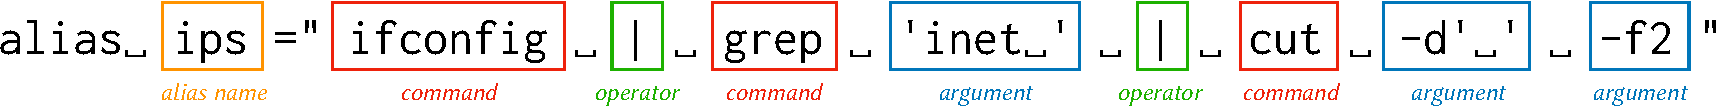
\includegraphics[width=0.85\textwidth]{parser_breakdown.pdf}
    \caption{Example decomposition of an alias definition.}
    \label{fig:parser}
\end{figure*}

The decomposed aliases are stored in the same SQLite database as the raw file contents, to facilitate easy cross-referencing.
The database schema is given in \cref{fig:schema}.
Files that did not contain any aliases were removed from the database after parsing, as was repository metadata that only referenced files without aliases.

\begin{figure}
    \centering
    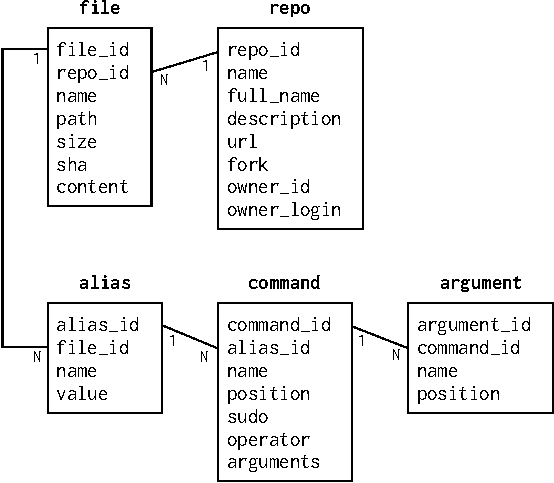
\includegraphics[width=0.9\columnwidth]{schema.pdf}
    \caption{Relational database schema.}
    \label{fig:schema}
\end{figure}

\subsection{Reproducibility}

To enable reproducibility and follow-up studies, we have made all data and our entire tool-chain publicly available.
This includes executable Jupyter notebooks used during our analysis, containing all SQL queries and Python code.
Our entire database (\TODO GB), the parsing script (written in Haskell), the notebooks, as well as this paper, are available on GitHub\footnote{\TODO: url}.

